\section{An Improved Model for the Evolution of $Q_\mathrm{H\,II}$}
\label{Qdot}

In this section we compare the evolution of the ionized volume fraction $Q_\mathrm{H\,II}$ from our simulation with the analytic model introduced by \cite{MadauEtAl1999}. We are motivated to do this because as we have seen from \S\ref{sec:ClumpingFactors}, Equation \eqref{eq:ndot} is not a useful predictor of when $Q_\mathrm{H\,II}$ reaches unity. We therefore want to investigate the accuracy of the time dependent model from which Equation \eqref{eq:ndot} is derived as a limiting case.

 \cite{MadauEtAl1999} derived the following ODE for the evolution of $Q_\mathrm{H\,II}$ (their Equation 20):

%After our initial investigation into the accuracy of Equation \eqref{eq:updatedNdot} for determining the end of EoR, we want to try probe the validity for the equation that determines the volume filling fraction of H {\footnotesize II}.  The algebraic form of Equation (23) in \citep{MadauEtAl1999} should determine the volume filling fration of ionized region, but it is derived with assumptions from the differential form.  Without taking simplifying steps, the differential form is Equation (20) \citep{Madau1999},

\begin{equation}
	\label{eq:dQdt}
	\frac{dQ_\mathrm{H\,II}}{dt} = \frac{\dot{n}_{ion}}{\bar{n}_\mathrm{H}}-\frac{Q_\mathrm{H\,II}}{\bar{t}_{rec}}
\end{equation}
where $\dot{n}_{ion}$ is ionizing photon injection rate, $\bar{n}_\mathrm{H}$ is the mean density of H atoms in the universe, and $\bar{t}_{rec}$ is some characteristic recombination time taking the clumpiness of the IGM into account. For a constant clumping factor and comoving emissivity \cite{MadauEtAl1999} show that 
\begin{equation}
Q_\mathrm{H\,II}(t) \approx \frac{\dot{n}_{ion}}{\bar{n}_\mathrm{H}} \bar{t}_{rec}
\end{equation}
Setting $Q=1$ one arrives at  $\dot{n}_{ion}\bar{t}_{rec}=\bar{n}_\mathrm{H}$, the basis for deriving Equation \eqref{eq:ndot}. \cite{MadauEtAl1999} state that this relation should still be valid provided the clumping factor and comoving emissivity are slowly varying on a timescale of $\bar{t}_{rec}$. We utilize the differential form for our comparison because our emissivity is not a constant value, nor is it slowly varying on a recombination time as $Q \rightarrow 1$, as we show below.  %so the subsquent simplification to get the differential form to the algebraic form is invalid for us.  
%The differential form is shown as Equation \eqref{eq:dQdt}, where $Q$ is the volume filling fraction, $t$ time, $\dot{n}_{ion}$ the number of ionizing photon production rate density, $\bar{n_\mathrm{H}}$ the volume averaged number density of hydrogen atoms, and $t_{rec}$ is the recombination time, which we now investigate.

A practical issue when testing Equation \eqref{eq:dQdt} is how $\bar{t}_{rec}$ should be evaluated when $Q<1$, and in particular when $Q\ll 1$. In the limit $Q\ll 1$ one is dealing with isolated H {\footnotesize II} regions evolving under the influence of local conditions. Yet the definition for $\bar{t}_{rec}$ in Equation \eqref{eq:tmadau} invokes {\em global} values for $C$ and $\langle n_\mathrm{H\,II} \rangle$. Should these quantitles be evaluated locally only within ionized regions? Or are global estimates good enough? In particular, since \cite{MadauEtAl1999}'s Equation (20) uses $\bar{n}_\mathrm{H}$ as a proxy for $\langle n_\mathrm{H\,II} \rangle$, what is the appropriate value for $C$ to use?

A second practical issue is what to take for $\dot{n}_{ion}$. This is commonly understood to be the rate at which ionizing photons are injected into the IGM (e.g., Haardt \& Madau 2012, \S9.3), which in our parlance is $\dot{N}_{IGM}$. Or should we take the actual ionization rate density measured in the simulation $\dot{N}_t$? As we saw in the previous section, these two rates diverge as overlap is approached, and differ by more than an order of magnitude after overlap (Fig. \ref{Ndot_Ratio}). 

To examine these issues we plot in Figure \ref{Qeffv1} $Q(z)$ from our simulation, as well as theoretical curves obtained by integrating Equation \eqref{eq:dQdt} under various assumptions. The curve labelled $Q(sim)$ is the ionized volume fraction from our simulation that is at least 99.9\% ionized (Well Ionized). The other four curves are obtained by integrating Equation \eqref{eq:dQdt} setting $\dot{n}_{ion}=\dot{N}_t$ for various choices for $\bar{t}_{rec}$ (we investigate the $\dot{n}_{ion}=\dot{N}_{IGM}$ case at the end of this section.) The integral is approximated by summing a piecewise linear interpolation of the two terms on the RHS of Equation  \eqref{eq:dQdt} using the trapezoidal rule:
\begin{align}
Q(t) &= \int_{t*}^{t} \frac{dQ}{dt}dt \approx \sum \frac{dQ}{dt} \Delta t \notag\\
&= \sum_{i}(\mathrm{Term_1} - \mathrm{Term_2})_i \Delta t_i
\label{eq:integration}
\end{align}
where $t*$ is the time when the first star forms in the simulation.

The curve labeled $Q(\langle t_{rec}\rangle)$ uses the volume averaged recombination time (volume average of Equation \ref{recombtime}).  The two curves labeled $Q(t_\mathrm{Madau})$ use Equation \eqref{eq:tmadau} to evaluate $\bar{t}_{rec}$ for $C=2$ and $3$, substituting $\bar{n}_\mathrm{H}$ for $\langle n_\mathrm{H\,II} \rangle$ and assuming a constant T=10$^4$K for the IGM. 
%is using the definition of $\bar{t_{rec}}$ in \cite{MadauEtAl1999}, which is using the volume averaged number density of H {\footnotesize II} along with the clumping factor as $[(1+2\chi)\langle n_\mathrm{H\,II}\rangle \alpha_\mathrm{B} C]^{-1}$, assuming a constant T=10$^4$K which gives $\alpha_B\sim2.59\times10^{13}$cm$^{-3}$s$^{-1}$ in the IGM.  
The curve labeled $Q(t_{rec,eff})$ uses the effective recombination time definition 
\begin{equation}
	\label{eq:treceff}
	\bar{t}_{rec}=t_{rec,eff}\equiv \frac{\langle n_\mathrm{H\,II}\rangle}{\langle n_\mathrm{H\,II} n_e \alpha_B(T)\rangle}
\end{equation}
This particular definition makes the last line of Equation \eqref{eq:trecpart2} true trivially, with no assumption about the IGM temperature or ionization state of the hydrogen.  It involves no {\em ad hoc} clumping factors, and represents the actual appropriately averaged recombination time in the simulation. All the above volume averaged quantities have the threshold of $\Delta_b<100$ applied, and thus exclude dense gas bound to halos.   
%The curve $Q(sim)$ is the actual ionized volume fraction to Well Ionized level vs. z.  
Several of the curves derived from integrating $\frac{dQ}{dt}$ reach values above unity at the end of the overlapping phase. While it is physically impossible to have $Q>1$ it is not mathematically forbidden, and so we show the complete curves because they give us some insight about the relative contribution of the recombination term (Term$_2$) as compared to the ionization term (Term$_1$).

The $Q(\langle t_{rec}\rangle)$ curve ionizes the quickest, reaching  $Q=1$ at $z\sim 6.5$, which is substantially before the simulation which achieves it at $z\approx 5.8$. The reason for this, as we will analyze shortly, is that recombinations play essentially no role in this model. The $Q(t_{rec,eff})$ curve has the same shape as the $Q(sim)$, but is everywhere higher, and crosses $Q=1$ at $z\sim 6.1$. Given that this integration uses the actual ionization rate density and effective recombination time in the simulation, this discrepancy demands an explanation. We address this below. Finally the $Q(t_\mathrm{Madau})$ curves do not match the shape of the $Q(sim)$ curve, ionizing more quickly at early times, and exhibiting a maximum value for $Q$ at $z \sim 6$. 

\begin{figure}
    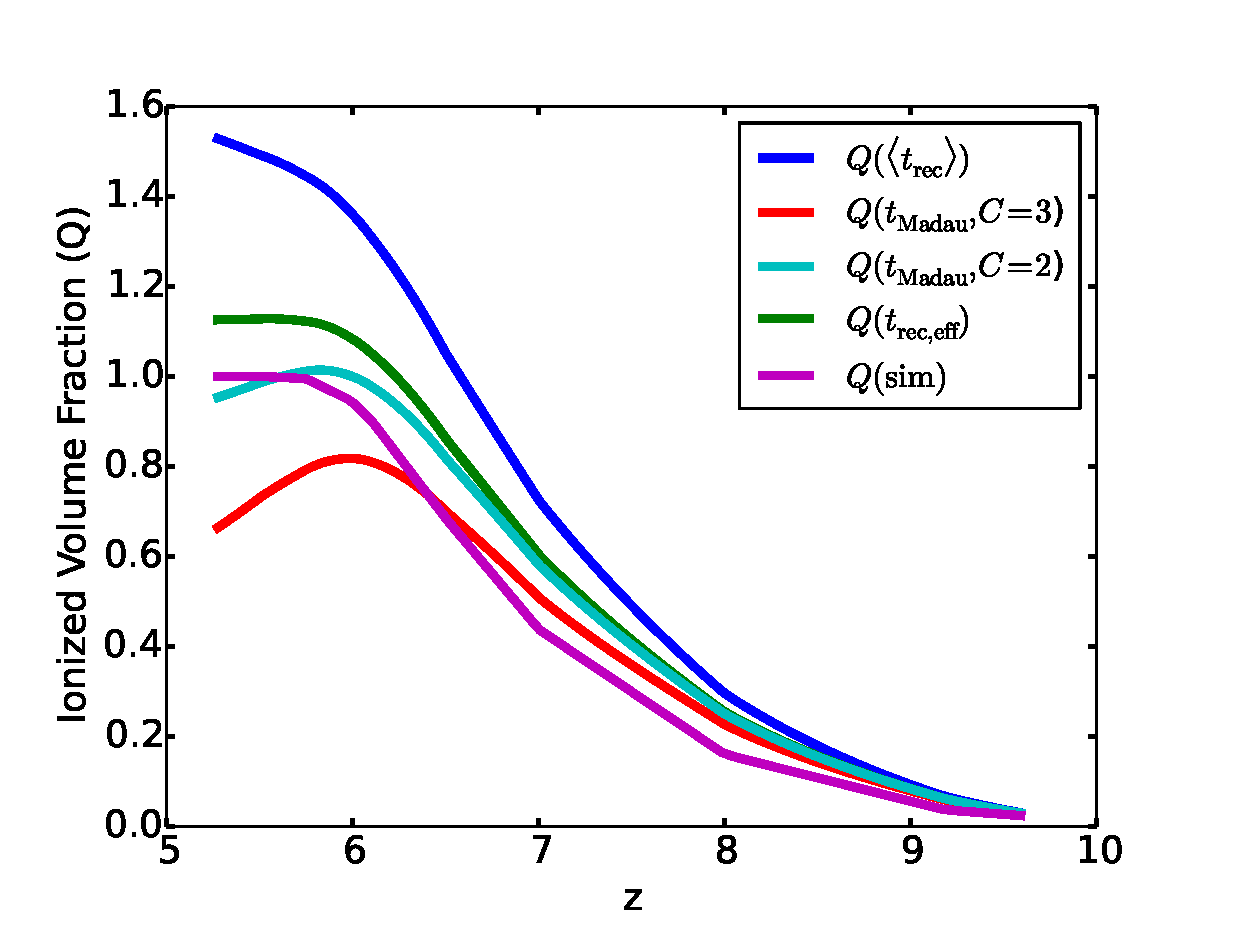
\includegraphics[width=0.5\textwidth]{Qeffv1.eps}
    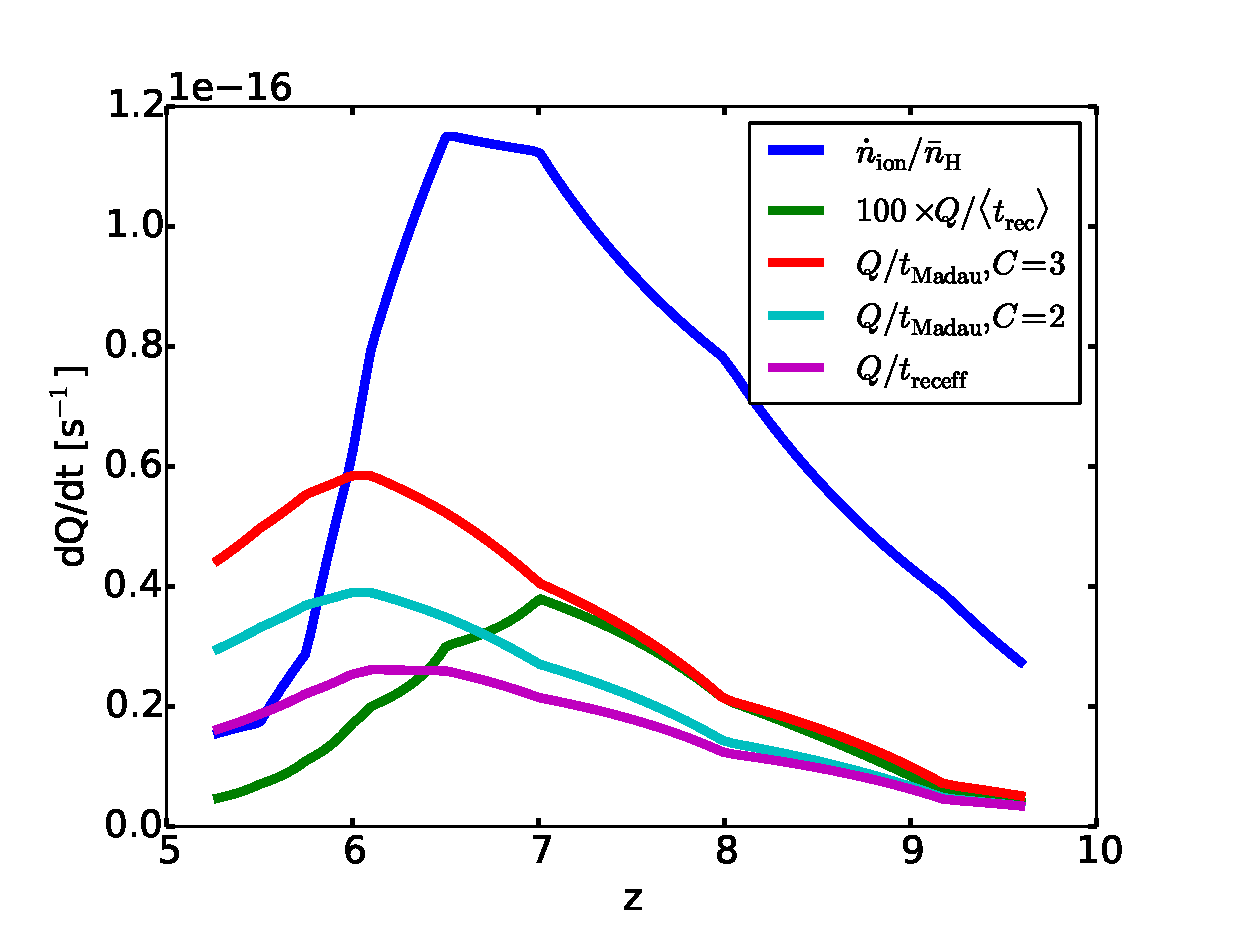
\includegraphics[width=0.5\textwidth]{term1vsterm2.eps}
    \caption{{\em Top}: Comparison of the evolution of the ionized volume fraction Q from our simulation with the analytic model introduced by \cite{MadauEtAl1999}.  Q(sim) is calculated directly from counting the cells satisfying the Well Ionized threshold of $f_i>0.999$. The other curves are calculated from integrating Equation \eqref{eq:integration} with the different expressions for $\bar{t}_{rec}$ in Term$_2$, as described in the text.  {\em Bottom}:  Plot of Term$_1$ and Term$_2$ individually using the different expressions for $\bar{t}_{rec}$.}
    \label{Qeffv1}
\end{figure}

To understand this behavior more fully we plot in Figure \ref{Qeffv1} {\em bottom} the values for Term$_1$ and Term$_2$ in Equation \eqref{eq:dQdt}. 
%We are curious as to why the integrated curves reach values above unity, so we look at the relative contribution of each of the two terms in Equation \eqref{eq:dQdt}, and we plot the result in Figure \ref{term1vsterm2}.  
The blue curve is Term$_1$ of Equation \eqref{eq:dQdt}. The other four curves plot Term$_2$ with their respective values for $\bar{t}_{rec}$.  The ionization curve dominates all the recombination curves at high redshifts, and reaches a maximum at $z\sim 6.5$. 
This is a partial reflection of the plateauing and subsequent decline of the SFRD shown in Figure \ref{SFR}. More fundamentally, it is a reflection of the rapid drop in the neutral fraction of the IGM as overlap is approached.  
%The physical reason for this is the suppression of star formation in low mass halos post-reionization, which is the topic of a future paper in this series.  
The curve using the volume averaged recombination time $\langle t_{rec}\rangle$ yields such low values compared to the others that we multiply it by 100 to make it more visible.  Although this is not the relevant recombination time to use, since it weights low density regions, it is effectively the limiting case $\bar{t}_{rec}\rightarrow \infty$.  We can therefore interpret the blue curve in Figure \ref{Qeffv1}a as an integration of the ionization term only. It is significantly higher than the $Q(sim)$ curve, suggesting that recombinations are important in the simulation at some level. The ionization term dominates the recombination term by factors of $6-10$ in the $t_{rec,eff}$ curve until just before overlap, and the two terms come into balance after overlap. The two $t_\mathrm{Madau}$ recombination curves are subdominant to the ionization term until $z \sim 6$, and at lower redshifts they become dominant. This explains the turnaround in the corresponding $Q$ curves in Figure \ref{Qeffv1}a. 

The differences in the magnitude of the recombination curves in Figure \ref{Qeffv1}b, especially at higher redshifts, is directly attributable to the magnitude of $\bar{t}_{rec}$. For completeness we plot $\bar{t}_{rec}$ versus redshift in Figure \ref{treceffhubble}, both unnormalized and normalized by $t_\mathrm{Hubble}$. In addition to the three curves for $t_{rec,eff}$ and $t_\mathrm{Madau}$ for $C=2, 3$, we also plot $t_\mathrm{Madau}$ for $C=C_\mathrm{ttH\,II}$ and $C=C_\mathrm{tdm}$. We see that all the curves with the exception of the Madau formula curve using the thresholded dark matter clumping factor exhibit an increasing recombination time with decreasing redshift, in line with our expections. The latter curve shows the opposite trend, which is due to the fact that the dark matter clumping factor increases with decreasing redshift, even if it is thresholded to exclude halos (see Figure \ref{thresholded} bottom). Among the remaining curves the $t_{rec,eff}$ has the highest values, and increases more sharply than the $t_\mathrm{Madau}$ curves due to the temperature of the IGM. To demonstrate that, we plot one additional curve (dashed curve) for $t_{rec,eff}$ evaluated assuming a constant $T=10^4$K in the recombination rate coefficient.

We now comment on the often-made assumption in reionization models that $\bar{t}_{rec} \ll t$. \cite{MadauEtAl1999} make this assumption in order to derive Equation \eqref{eq:ndot}. It is this assumption that allows for an instantaneous analysis of the photon budget to maintain the universe in an ionized state while ignoring history dependent effects.
Referring to  Figure \ref{treceffhubble}b we see this is never true for $t_{rec,eff}$ and it is not true for $t_\mathrm{Madau}$ at redshifts approaching overlap for any sensible value of $C$. We therefore conclude that history-dependent effects cannot be ignored, and that this is the reason Equations \eqref{eq:ndot}, \eqref{eq:updatedNdot} and \eqref{eq:ShullNdot} mis-predict the epoch of reionization completion. For the same reason applying these formulae at lower redshifts is highly suspect.  

%Clearly, the first term is dominant over different versions of the second term.  However, the second term with $Q/t_{rec,eff}$ is not negligible, and contributes the most by having recombination curb the growth of $Q$ from the first term.

%\begin{figure}
%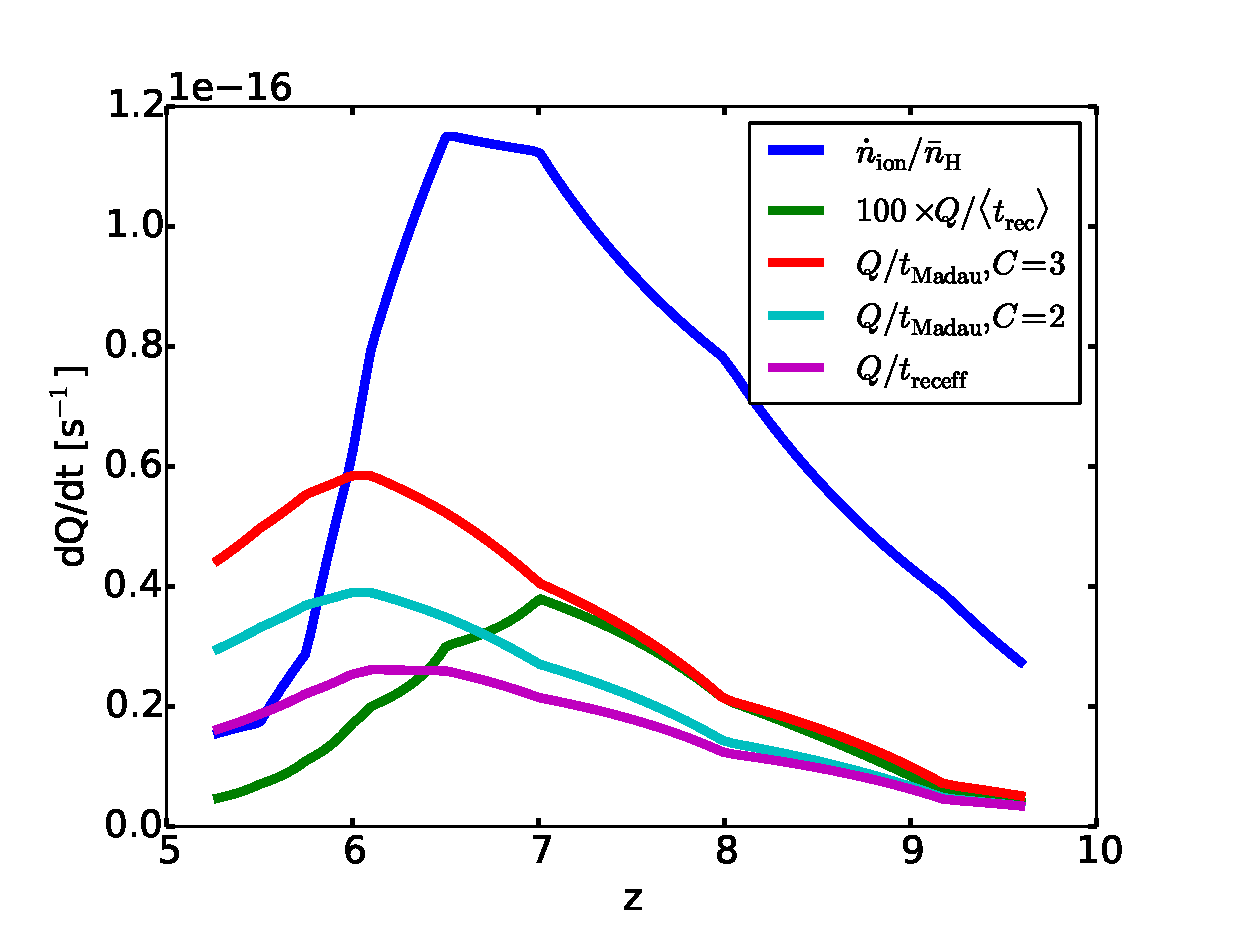
\includegraphics[width=0.5\textwidth]{term1vsterm2.eps}
%	\caption{test}
%\label{term1vsterm2}
%\end{figure}

%The best case scenario is represented by using $t_{rec,eff}$, and to focus on the difference, we plot each $t_{rec}$ with respect to the hubble time $t_\mathrm{Hubble}$ in Figure \ref{treceffhubble}.  This time, we multiply $t_{rec,eff}/t_\mathrm{Hubble}$ by a factor of 100 to maintain visibility along with the other two curves.  The figure shows $t_{rec,eff}$ to be the lowest, which tells us that recombinations are happening on a quicker time scale using this definition as oppose to other definitions.  Also notice that the other two curves with $\rangle t_\mathrm{rec}\langle$ and $t_\mathrm{Madau}$ divided by $t_\mathrm{Hubble}$ both have values much greater than unity, therefore the assumptions made in \cite{MadauEtAl1999} that says only the instantaneous ionization rate is important and not its history is not valid here.  Even though the $t_\mathrm{rec,eff}$ curve started below 1.0, it is not an order of magnitude lower, and crosses above 1.0 around $z\sim 6.5$, so the claim $t_{rec} \ll t_\mathrm{Hubble}$ is never satisfied.

\begin{figure}
    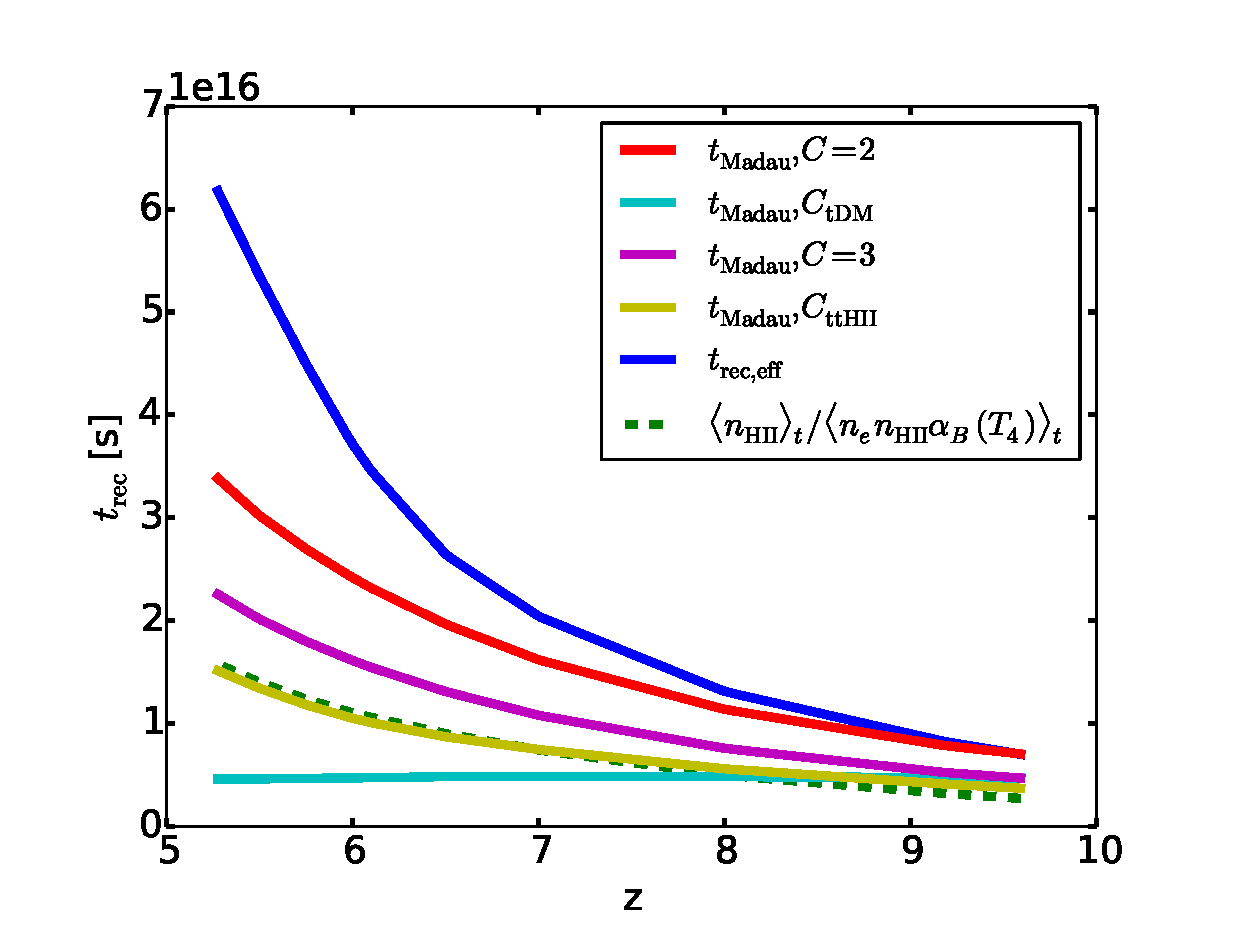
\includegraphics[width=0.5\textwidth]{tmisc.eps}
    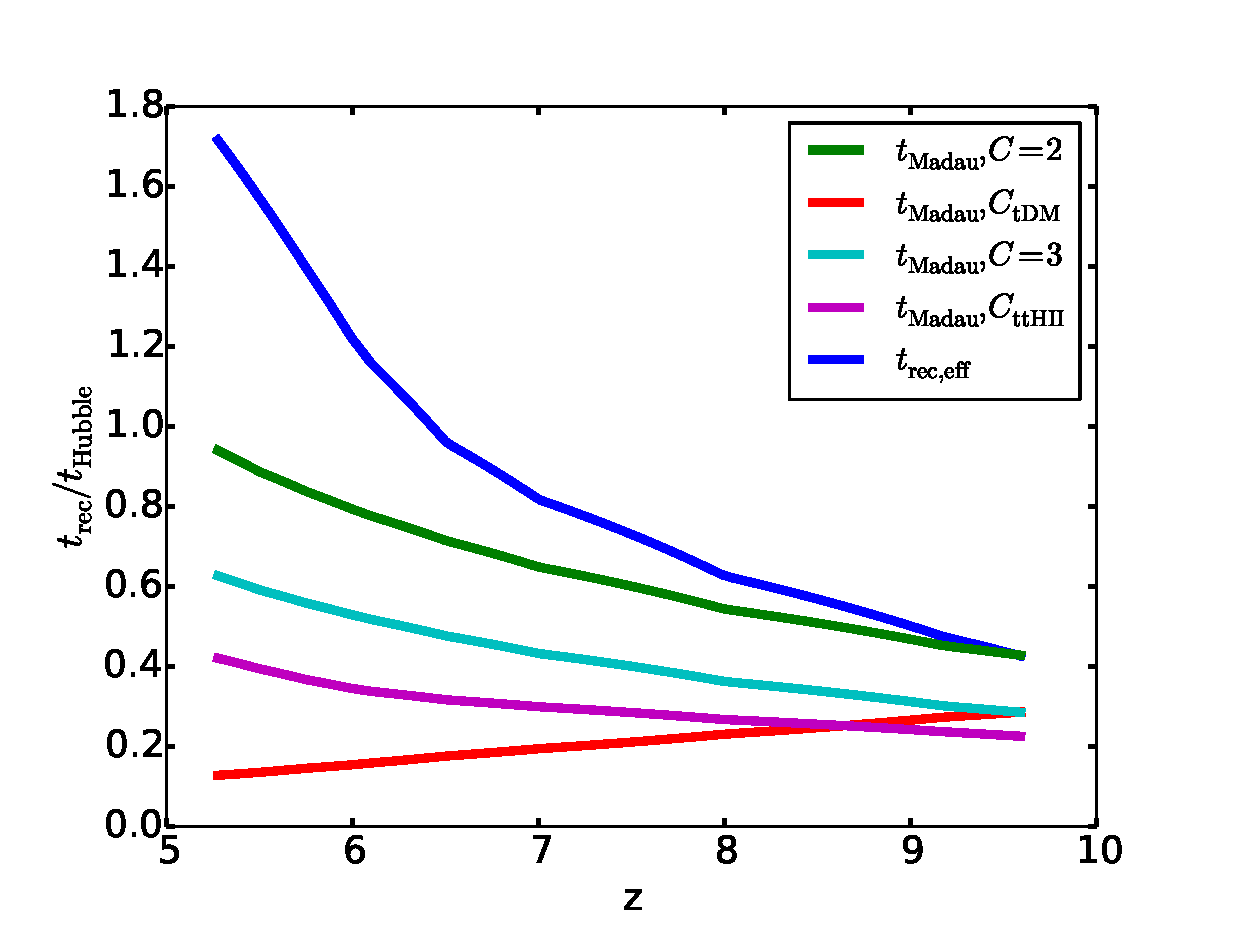
\includegraphics[width=0.5\textwidth]{treceffhubble.eps}
    \caption{{\em Top}: Recombination time versus redshift, for various expressions for $\bar{t}_{rec}$ as described in the text. Curve labeled $t_{rec,eff}$ is the characteristic recombination time measured directly in the simulation. Curves labeled $t_{Madau}$ evaluate Eq. \eqref{eq:tmadau} for various choices for the clumping factor C. {\em Bottom}: Recombination time versus redshift normalized by the Hubble time, for various expressions for $\bar{t}_{rec}$.}
    \label{treceffhubble}
\end{figure}

Returning to the discrepancy between the $Q(sim)$ and $Q(t_{rec,eff})$ curves in Figure \ref{Qeffv1}a, since the most sensible choice for $t_{rec}$ did not give us satisfactory agreement, we wondered what the origin of the discrepancy could be.  Since we have shown that recombinations are relatively unimportant at high redshifts, but that the discrepancy is already present at high redshifts, the only possibility is that there is something wrong with the first term of Equation \eqref{eq:integration}. When looking at the derivation for Equation \eqref{eq:dQdt} in \cite{MadauEtAl1999}, it is stated that it ``approximately holds for every isolated source of ionizing photon in the IGM.''  That got us to think that our calculation of $\bar{n}_\mathrm{H}$ may be off from what is originally intended if it is a global average over the entire simulation box.  Since the original $\frac{dQ}{dt}$ is derived from the analytical Str\"{o}mgren sphere model, it assumed a single ionizing source at the center of the volume, and the the average density of the box is just the uniform density everywhere, we thought that might be the discrepancy.  In an Inside-out model, I-fronts are not initially propagating in a gas with an average density given by $\bar{n}_H$, but somewhat higher density. Would agreement improve if instead of using $\bar{n}_H$ in the first term of Equation \eqref{eq:dQdt}, we used the local average density?

%We attempt to use a $\delta_b\equiv \langle \rho_b\rangle_{tt}/\langle \rho_b\rangle_{t}$ as a correction factor to the right hand side term 1 in Equation \eqref{eq:dQdt}.  The volume average $\langle\rangle$ with subscript $t$ is the usual $\Delta_b<100$ threshold, the double subscript $tt$ indicates the additional threshold of $x>0.1$, therefore the correction factor $\delta_b$ tells us how much denser are the ionized gas that the radiation front has passed through, compare to the rest of the box.  The denser average number density of hydrogen will be enhanced by a factor of $\delta_b$ as follows:

We therefore modify Equation \eqref{eq:dQdt} as follows:
\begin{equation}
	\frac{dQ}{dt} = \frac{\dot{n}_{ion}}{\delta_b\bar{n}_\mathrm{H}}-\frac{Q}{\bar{t}_{rec}}
	\label{eq:dQdtdb}
\end{equation}
where we have introduced in the denominator of the first term a factor $\delta_b \geq 1$ which corrects for the higher mean density within ionized bubbles. We measure $\delta_b$ from each redshift output as follows: $\delta_b = \langle \rho_b\rangle_{tt}/\langle \rho_b\rangle_{t}$. The volume average $\langle\rangle$ with subscript $t$ is the usual $\Delta_b<100$ threshold, the double subscript $tt$ indicates the additional threshold of $x_e>0.1$. Thus $\delta_b$ is the average baryon overdensity within Ionized regions excluding gas inside halos. Figure \ref{deltabvsQfit5} shows a plot of $\delta_b$ versus $Q$ together with a simple fitting formula which fits the data extremely well over the domain $0.01 \leq Q \leq 1$. 

To see if this formulation improves agreement with our simulated data, in Figure \ref{Qeffv2} we integrate Equation \eqref{eq:dQdtdb} again setting $\dot{n}_{ion}=\dot{N}_t$ and using $t_{rec,eff}$ to evaluate the second term. For comparison we show the curve obtained setting $\delta_b=1$, which repeats a curve already presented in Figure \ref{Qeffv1}.  Although the simulated and integrated analytic model curves do not agree exactly, the $Q(\delta_b,t_{rec,eff})$ curve shows much better agreement with the simulation, with error on the order of 1\% instead of 10\%.

\begin{figure}
	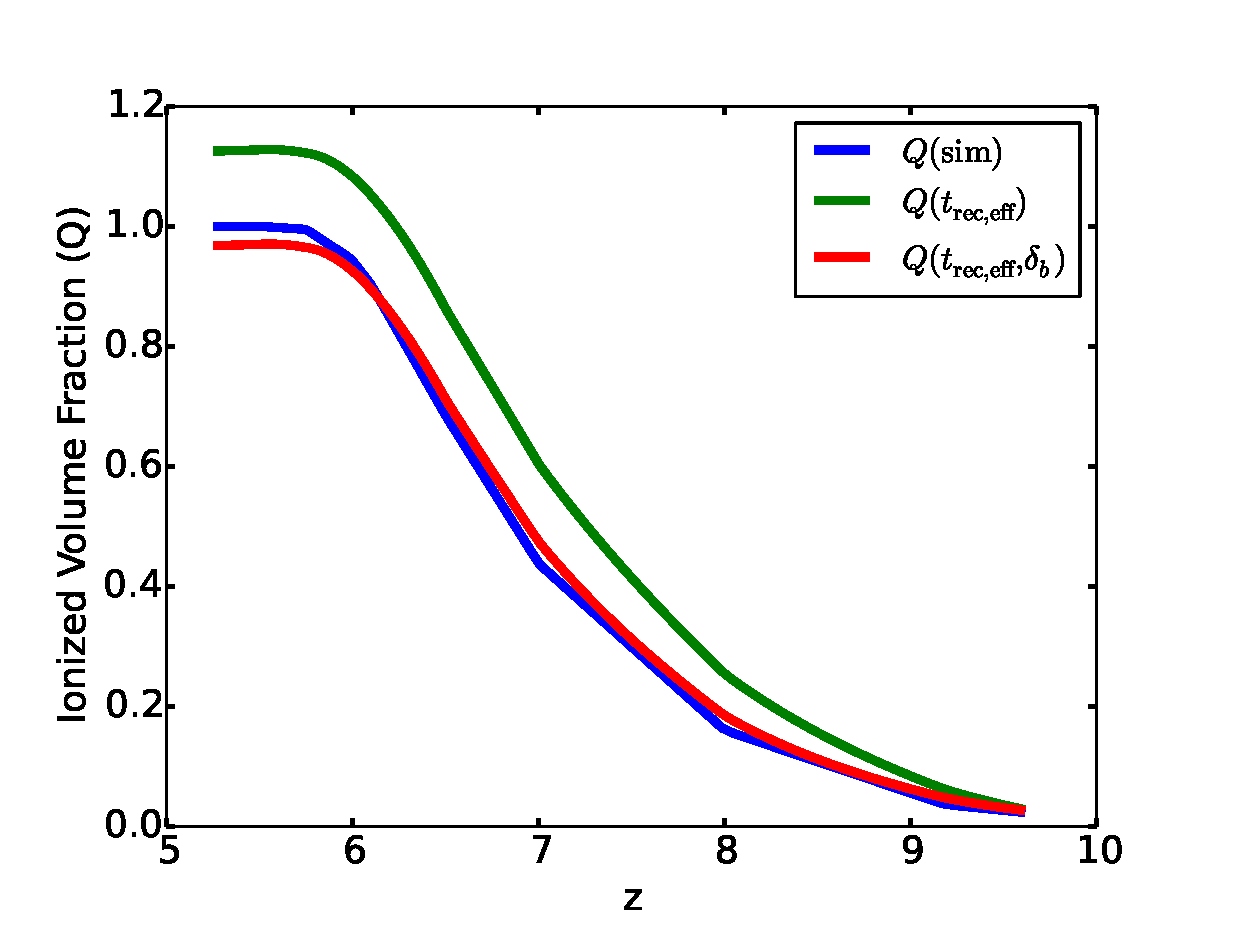
\includegraphics[width=0.5\textwidth]{Qeffv2.eps}
	\caption{Improved agreement between theory and simulation. Green and blue curves are as in Fig. \ref{Qeffv1}. Red curve is obtained by integrating modified evolution equation for Q taking into account the overdensity effect of Inside-out reionization (Equation \eqref{eq:dQdtdb}).}
	\label{Qeffv2}
\end{figure}

By not assuming a constant emissivity and using the modified differential form in determining the volume filling fraction of Equation \eqref{eq:dQdtdb}, we are able to more accurately model the evolution of the simulated volume filling fraction of H {\footnotesize II} to the Well Ionized level. For completeness we plot in Figure \ref{treceffvszfit} the evolution of $t_{rec,eff}$ used in the above integration, including a reasonably good fit to the data. 

%For the volume filling fraction of H {\footnotesize II} $Q$, we are able to get a good agreement ($\sim O(1\%)$) with simulation using slight modification to the differential equation resulting in Equation \eqref{eq:dQdtdb}.  Even though the volume fraction is originally derived for a single radiating source in a uniform medium, we were able to modify it for the cosmological case.  We believe by using $\delta_b$ we are considering a more representative gas density that is actually affected by the radiation, and using $t_{rec,eff}$ is a more accurate representation of the recombination time for the hydrogen being ionized in the IGM.  Here we show the simple fitting formula for $\delta_b$ and $t_{rec,eff}$ respectively as Figure \ref{deltabvsQfit5} and \ref{treceffvszfit}.

\begin{figure}
	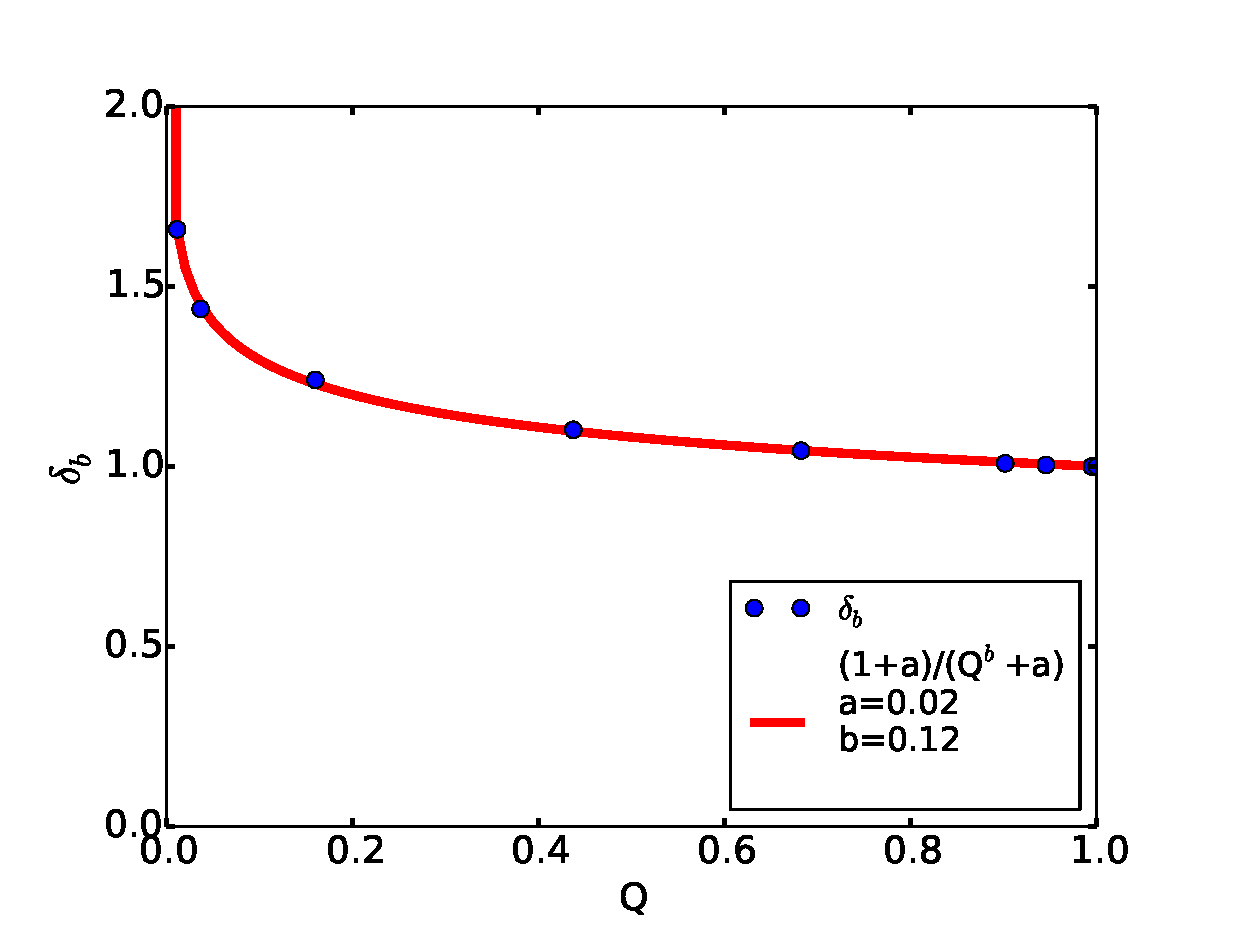
\includegraphics[width=0.5\textwidth]{deltabvsQfit5.eps}
	\caption{Mean baryon overdensity of ionized gas as a function of the ionized volume filling fraction Q. Blue points are measured in the simulation by averaging over the doubly thresholded cells obeying $\Delta_b<100$ and $x_e > 0.1$. Red curve is a fit to the data.}
	\label{deltabvsQfit5}
\end{figure}

\begin{figure}
	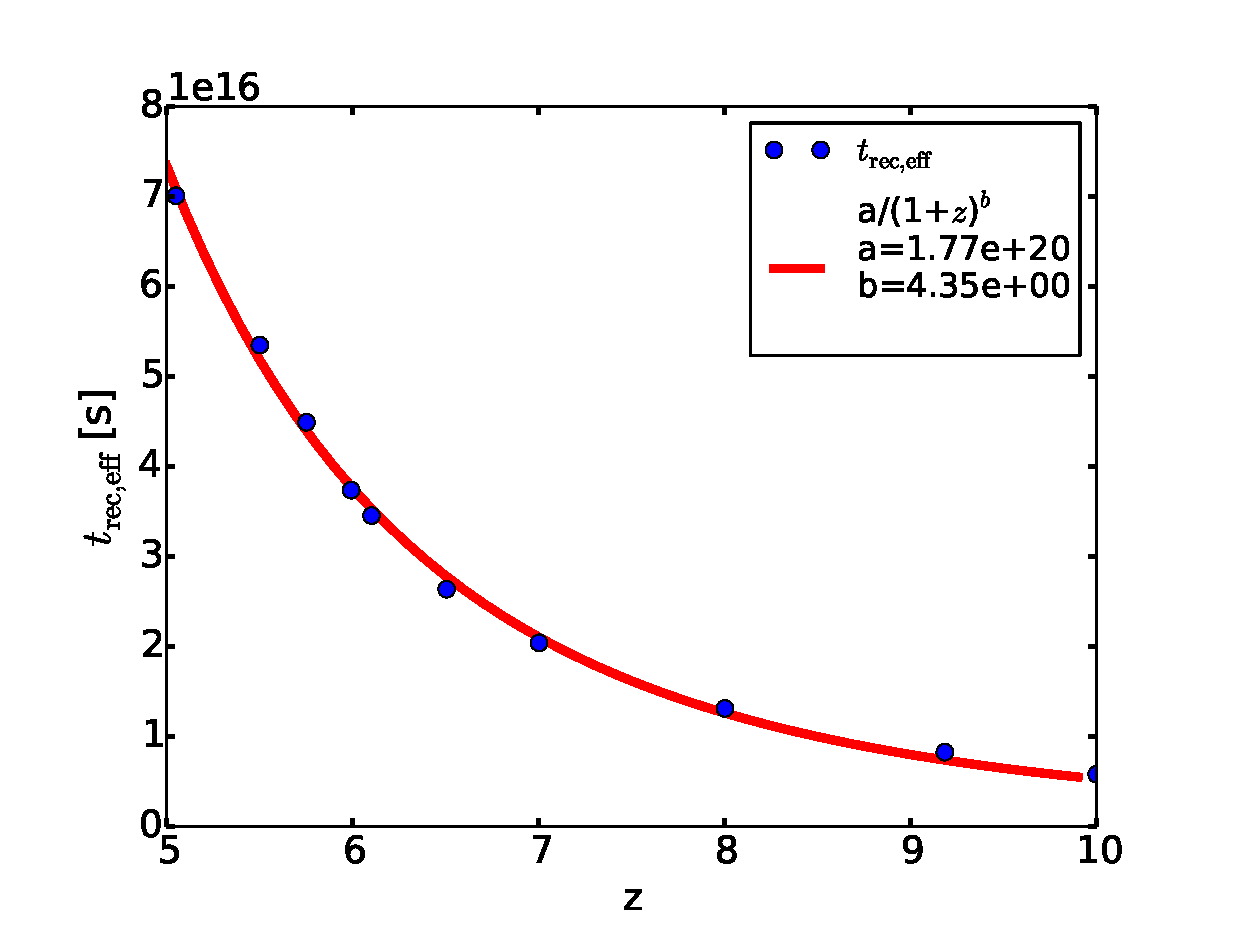
\includegraphics[width=0.5\textwidth]{treceffvszfit.eps}
	\caption{Analytic fit to $t_{rec,eff}$ (red line) , evaluated using simulation data (blue points) via Equation \eqref{eq:treceff}.}
	\label{treceffvszfit}
\end{figure}

Finally, we return to the question of what is the appropriate choice for $\dot{n}_{ion}$ in Equation \eqref{eq:dQdtdb}. This is commonly taken to be the rate at which ionizing photons are injected into the IGM (e.g., Haardt \& Madau 2012, \S9.3), because this can be connected to the observed UV luminosity density $\rho_{UV}$ by the formula $\dot{n}_{ion}=f_{esc}\xi_{ion}\rho_{UV}$, where $f_{esc}$ is the escape fraction for ionizing radiation, and $\xi_{ion}$ is the rate of ionizing photons per unit UV (1500 \AA{}) luminosity for the stellar population \citep{RobertsonEtAl2013}. However we have obtained excellent agreement between simulation and Equation \eqref{eq:dQdtdb} using the mean ionization rate density in the IGM  $\dot{N}_t$, which differs from the ionizing photon injection rate density $\dot{N}_{IGM}$ as $Q \rightarrow 1$. In Figure \ref{Qeffv3} we show the result of integrating Equations \eqref{eq:dQdt} and \eqref{eq:dQdtdb} with the choice $\dot{n}_{ion}=\dot{N}_{IGM}$, as originally proposed by \citep{MadauEtAl1999}. Also plotted in Figure \ref{Qeffv3} is $Q(sim)$ (blue line) and our best agreeing model (green line). The red line ignores the $\delta_b$ correction, and deviates to the high side of $Q(sim)$ almost immediately, for reasons we discussed earlier. It crosses $Q=1$ at $z\approx 6.6$, which is too early by $\Delta z =0.8$. The teal line includes the $\delta_b$ correction, and tracks the $Q(sim)$ closely to $z \approx 7$, and thereafter deviates on the high side. It crosses $Q=1$ at $z\approx 6.4$, which is too early by $\Delta z =0.6$. Both curves show an accelerated change in $Q$  as z decreases, which is characteristic of standard analytic ionization models (e.g., Haardt \& Madau 2012, Fig.14). By contrast, the simulation and our best fit model using $\dot{n}_{ion}=\dot{N}_t$ show a decelerated change in $Q(z)$ as $Q \rightarrow 1$. This is clearly due to the fact that the ration of ionizations to emitted photons decreases as $Q \rightarrow 1$, as illustrated in Figure 22. The consequence of this flattening in the $Q(z)$ curve is a delay in redshift of overlap of $\Delta z=0.6-0.8$, relative to the predictions of Equations \eqref{eq:dQdtdb} and \eqref{eq:dQdt}, respectively, using the photon injection rate as the source term. 

We have seen above that the ionization rate density is the appropriate quantity to use to source the $dQ/dt$ equation, independent of $\delta_b$ corrections. Because the ionization rate density is not directly observable, but since $\dot{n}_{ion}$ can be derived from observables, we introduce a correction factor to convert from one to the other. Defining 
\begin{equation}
\gamma \equiv \frac{\langle n_{HI}\Gamma_{HI}^{ph}\rangle}{\dot{n}_{ion}} = \frac{\dot{N}_t}{\dot{n}_{ion}}
\label{gamma}
\end{equation}
\\where the angle brackets denote an average over the singly thresholded volume (IGM), then we can recast Equation \eqref{eq:dQdtdb} into a form useful for observers:
\begin{equation}
	\frac{dQ}{dt} = \frac{\gamma\dot{n}_{ion}}{\delta_b\bar{n}_\mathrm{H}}-\frac{Q}{\bar{t}_{rec}}, 
	\label{eq:dQdtdbg}
\end{equation}
\\where $\gamma$ and $\delta_b$ are functions of $Q$. 
In Fig. \ref{RatiovsQfit} we plot data values for $\gamma(Q)$ taken from our simulation, as well as a simple powerlaw fit. The fit is not meant to be definitive, but merely illustrative. More simulations need to be performed under various circumstances, and better fits made, to see whether our $\gamma(Q)$ is approximately universal, or merely anecdotal. 

\begin{figure}
	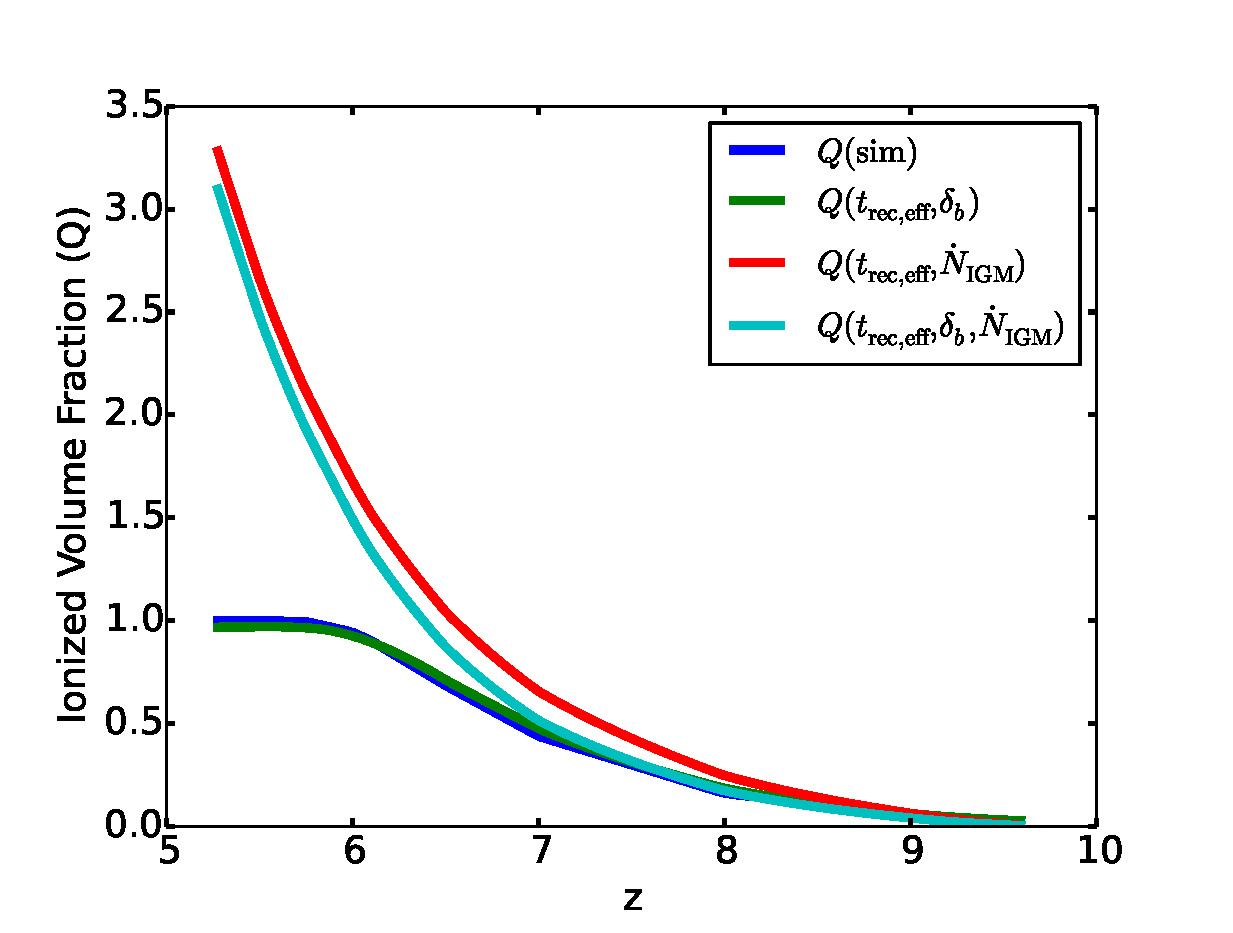
\includegraphics[width=0.5\textwidth]{Qeffv3.eps}
	\caption{Dependence of analytic models on the choice for $\dot{n}_{ion}$. Red and teal curves assume $\dot{n}_{ion}=\dot{N}_{IGM}$; i.e., the photon injection rate into the IGM. Green curve assumes $\dot{n}_{ion}=\dot{N}_{t}$; i.e., the measured photoionization rate in the IGM. Blue curve is $Q(sim)$--the measured ionized volume filling fraction in the simulation. The green and teal curves take into account the overdensity effect of inside-out reionization (Equation \eqref{eq:dQdtdbg}), while the red curve assumes $\delta_b=1$. All models assume $\bar{t}_{rec}=t_{rec,eff}$ as measured in the simulation (Fig. \ref{treceffvszfit}.}
	\label{Qeffv3}
\end{figure}

\begin{figure}
	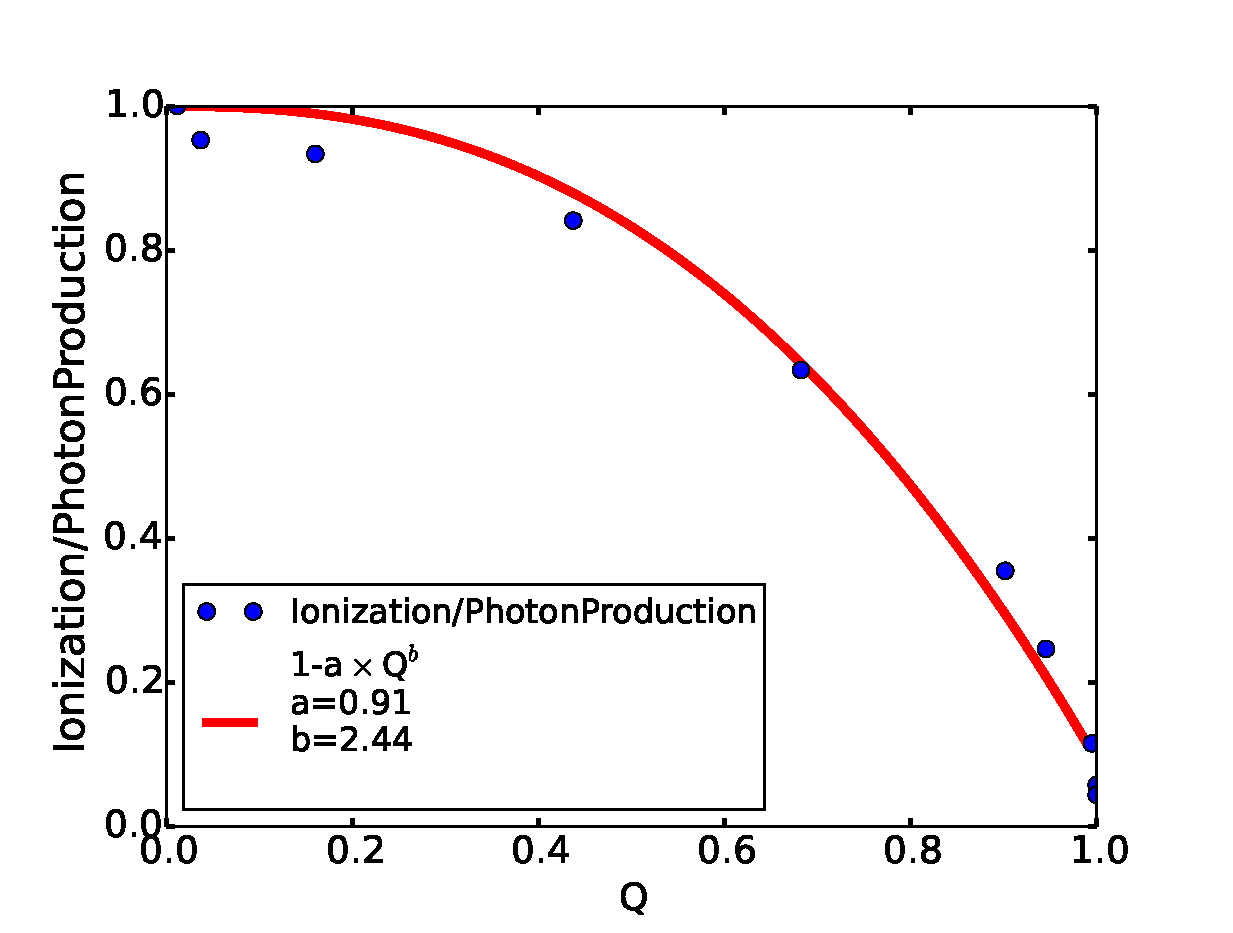
\includegraphics[width=0.5\textwidth]{RatiovsQfit.eps}
	\caption{Ratio of the volume averaged \hi photoionization rate to photon injection rate in the IGM as a function of $Q$. Data points are measured from the simulation; line is a simple powerlaw fit. }
	\label{RatiovsQfit}
\end{figure}

